%LV begin move all content to D10
%LV end move all content to D10

%LV begin insert content from D6

\chapter{Day 7: EVD and PCA}

\section{Schedule}
\bi
\item 0900-0930: Debrief
\item 0930-1015: Eigenvalue Decomposition (EVD)
\item 1015-1030: Coffee
\item 1030-1115: PCA and Maximum Variance
\item 1115-1210: Conceptual PCA and PCA blog post
\item 1210-1225: Review and Preview
\item 1225-1230: Survey
\ei

% \section{Benchmark Quiz [20 minutes]}
% Please figure out the answer to these questions and mark your answer in Canvas.

% \begin{enumerate}
% \item Which of the following is an eigenvalue and corresponding eigenvector of the matrix $\twobytwo{2}{2}{1}{3}$?
% \begin{enumerate}
% \item 1 and $\twobyone{-1}{2}$.
% \item 2 and $\twobyone{1}{1}$.
% \item 4 and $\twobyone{1}{1}$.
% \item 1 and $\twobyone{-\frac{1}{\sqrt 2}}{1}$.
% \end{enumerate}

% \item Consider a $2\times 2$ matrix $\A$ . The trace of $\A$ is 3 and the determinant of $\A$ is 2. What are the eigenvalues of $\A$?
%     \begin{enumerate}
%     \item 1 and 2
%     \item 2 and 3
%     \item -1 and 2
%     \item There is insufficient information to determine this.
%     \end{enumerate}

% \item Let $f(\x)$ be a function of a $2\times 1$ vector $\x$. This function is known to have a single critical point and the Hessian of $\x$ at the critical point is $\twobytwo{3}{1}{0}{2}$. Which of the following is true about the critical point of this function?
%     \begin{enumerate}
%     \item The critical point is a saddle.
%         \item The critical point is a local maximum.
%     \item The critical point is a local minimum.
%   \item The critical point is both a local minimum and a local maximum.
%     \end{enumerate}

% \item Consider the following scatter plots of data points with two variables. Suppose that the  eigenvalues of the covariance matrix of the data are 5 and 0.01, with the eigenvector corresponding to the largest eigenvalue being  $\twobyone{2}{1}$. Please find the scatter plot that has this characteristic.

% \begin{center}
% 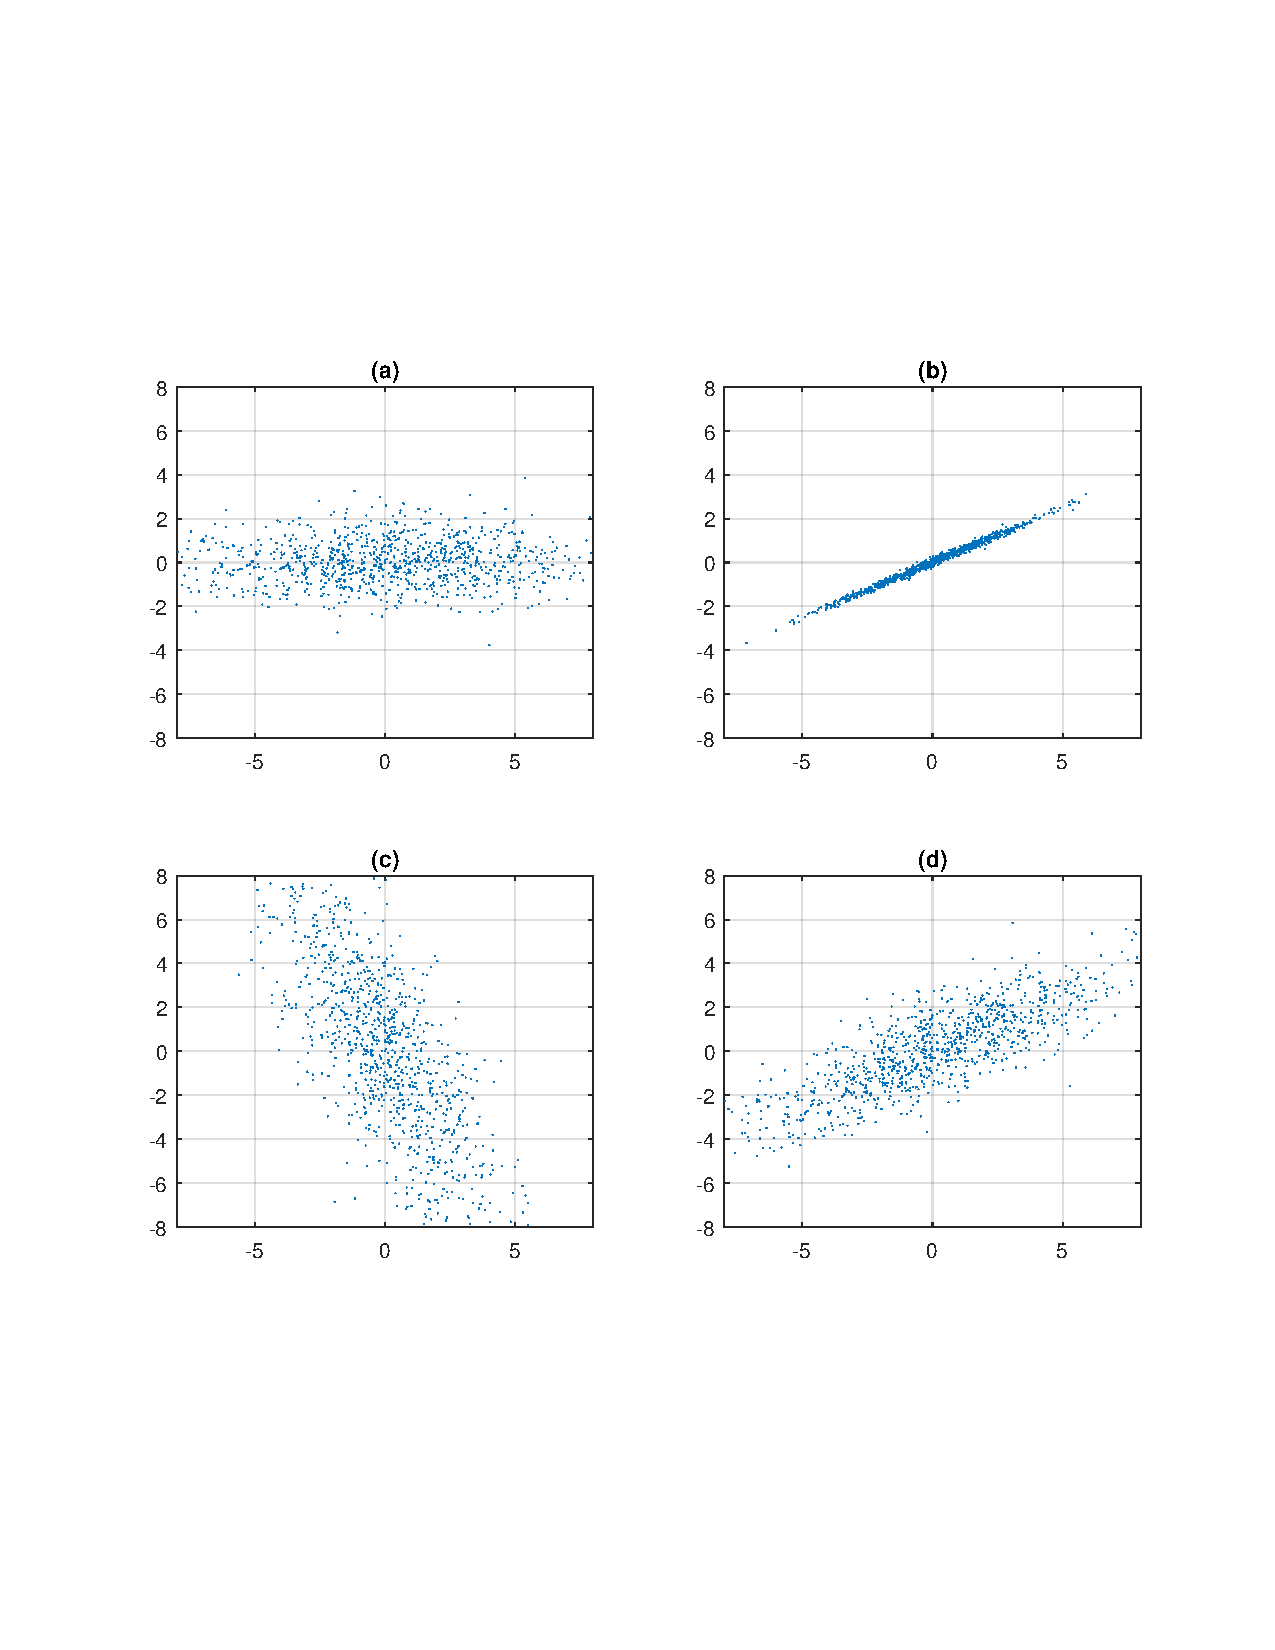
\includegraphics[width=0.75\textwidth]{FacesDay6/figs/Cov_illustration.pdf}
% \end{center}
% \end{enumerate}

% \clearpage

\section{Debrief [15 mins]}
In the last class and in the take-home exercise, you worked on a number of different exercises involving eigenvalues and eigenvectors. 

\begin{prob}
\begin{enumerate}
\item With your table, identify a list of key concepts/take home messages/things you learned in the last class and take-home assignment.
\item Try to resolve your confusions with the folks at your table and by talking to an instructor.
\end{enumerate}
\end{prob}

%\section{Basis vectors [15 mins]}
%
%The big idea of today is eigendecomposition, which we will use to generate a set of orthogonal vectors with certain desirable properties. These vectors will be used as basis vectors to express other vectors (namely vectors containing data) which can help us in a number of ways, including in face detection.  To get warmed up, please work on the following problem on the board with your table.
%
%\begin{enumerate}[resume]
%\item Consider a set of orthonormal vectors in 2 dimensions, $\twobyone{\frac{1}{\sqrt{2}}}{\frac{1}{\sqrt{2}}}$ and $\twobyone{-\frac{1}{\sqrt{2}}}{\frac{1}{\sqrt{2}}}$. Recall that that a set of vectors is orthonormal if they are orthogonal to each other and each have unit length.  Please write the vector $\twobyone{2}{3}$ as a linear combination of these basis vectors. By drawing appropriate vectors on the board, show how $\twobyone{2}{3}$ can be expressed as a sum of scaled versions of $\twobyone{\frac{1}{\sqrt{2}}}{\frac{1}{\sqrt{2}}}$ and $\twobyone{-\frac{1}{\sqrt{2}}}{\frac{1}{\sqrt{2}}}$.
%
%\item Consider the set of $n\times 1$ vectors $\v_1, \v_2, \cdots \v_n$. They define an orthonormal set if they are mutually orthogonal, and have unit norm. In other words,
%    \begin{align}
%    \v_i^T\v_i &= 1\\
%    \v_i^T\v_j &= 0 \mbox{ if } i\neq j\\
%    \end{align}
%    Let $\x$ some $n\times 1$ vector (we don't really need to know what it is specifically).
%    \begin{enumerate}
%    \item Is it possible to express $\x$ as a linear combination of the $\v_i$'s? In other words, are there values of $\alpha_1, \alpha_2, \cdots \alpha_n$ such that
%        \begin{align}
%        \x = \alpha_1\v_1 + \alpha_2 \v2 +\cdots + \alpha_n \v_n
%        \end{align}
%    \item If you answered in the affirmative to the previous question, please find $\alpha_i$ in terms of $\x$ and $\v_i$.
%    \end{enumerate}
%\end{enumerate}

%\clearpage

\section{Eigenvalue Decomposition (EVD) [45 mins]}

The eigenvalue decomposition, also known as the eigendecomposition, is an operation on matrices in which a square matrix is expressed as a product of matrices made up of its eigenvalues and eigenvectors.   It can be used to find inverses and powers of matrices, as well as to derive some important results in data analysis. For instance,  in a prior exercise, you saw that the eigenvector corresponding to the largest eigenvalue of a covariance matrix was in the direction of greatest variance in your data set. This property can be proved using the eigendecomposition.

The eigenvalue decomposition is also helpful in dimensionality reduction, which is a process where we can represent higher-dimensional vectors as a linear combination of a smaller number of vectors than dimensions -- an example of which you saw in a previous exercise where you represented pictures of peoples faces using a linear combination of vectors. The eigendecomposition is also often used to change coordinate systems.

\subsection{The Big Idea}

Assume that a square $n \times n$ matrix $\A$ has $n$ linearly independent eigenvectors $\v_i$ with corresponding eigenvalues $\lambda_i$, i.e.
\[\A \v_i = \lambda_i \v_i \; i=1,2,\ldots,n\]
%LV insert: I added a note to address some confusions that arose
% \todo[inline]{For the novice, I feel it is important to say, "It turns out these \textit{assumptions} are accurate for any square, symmetric matrix: their eigenvectors form an orthonormal basis." This is a good location to put a reflective question, "What are the properties of the resulting matrix, R, when multiplying a matrix, B, with its transpose, $B^T$?"}
%LV end insert
Instead of thinking of these eigenvalues and eigenvector separately, let's package them into matrices as follows:
\[[\A \v_1 \; \A \v_2 \; \ldots \; \A \v_n ] = [\lambda_1 \v_1 \; \lambda_2 \v_2 \; \ldots \; \lambda_n \v_n] \]
Properties of matrix multiplication suggests that we can re-write this matrix equation in the form
\[\A [\v_1 \; \v_2 \; \ldots \; \v_n ] = [\v_1 \; \v_2 \; \ldots \; \v_n ] \threebythree{\lambda_1}{0}{0}{0}{\ldots}{0}{0}{0}{\lambda_n}\]
where the last matrix has each eigenvalue on the diagonal. If we now define 
\begin{eqnarray*}
\mathbf{V} &=& [\v_1 \; \v_2 \; \ldots \; \v_n] \\
\mathbf{D} &=& \threebythree{\lambda_1}{0}{0}{0}{\ldots}{0}{0}{0}{\lambda_n}
\end{eqnarray*}
then the previous equation becomes
\[\A \mathbf{V} = \mathbf{V} \mathbf{D}\]
Since we assumed that the eigenvectors are linearly independent this implies that the columns of $\mathbf{V}$ are linearly independent which in turn implies that the inverse of $\mathbf{V}$ exists. We can there fore write
\begin{align}
\mathbf{A} = \mathbf{V}\mathbf{D}\mathbf{V}^{-1}\, 
\label{eqnEvalDecomposition}
\end{align}
where the matrix $\mathbf{V}$ has the $i$-th eigenvector of $\mathbf{A}$ as its $i$-th column, and $\mathbf{D}$ is a diagonal matrix with the $i$-th eigenvalue of $\mathbf{A}$ as its $ii$-th entry. This expression is known as the \textit{eigendecomposition} of $\A$.
\todo[inline]{I think it would help here to say, something like, "This expression is the same for any square, invertible matrix. An eidgendecomposition tells you that the original matrix is 'composed' of an eigenbasis with associated eigenvalues in D. There may come a time when it is more convenient to work in A's eigenbasis and then transform the result." }
In the special case where $\A$ is symmetric, the eigenvalues are real, and the eigenvectors are mutually orthogonal so that
\begin{eqnarray*}
\mathbf{V}^{-1}  = \mathbf{V}^{T} \,, \label{eqn:OrthSymmetry}
\end{eqnarray*}
which is a property of $n\times n$ matrices whose column vectors are mutually orthogonal and have a length of 1 (i.e., the column vectors are orthonormal).

\begin{prob}
\begin{enumerate}
\item Consider the following $2\times 2$ matrix $\mathbf{A}$.\begin{align*}
\mathbf{A} =
\begin{bmatrix}
2 & 1 \\
1 & 2
\end{bmatrix}
\end{align*}
By hand, compute its eigenvectors and eigenvalues, determine the matrices $\mathbf{V}$, $\mathbf{D}$, and $\mathbf{V}^{-1}$, and confirm that \eqref{eqnEvalDecomposition} is correct. Use MATLAB to confirm your results by computing >> [V,D]=eig(A). \textbf{Note}: you should normalize each of your eigenvectors to be unit length.
\ee
\end{prob}
\begin{sol}
\be
    \item The eigenvalues are $\lambda_1 = 1$ and $\lambda_2=3$ with corresponding eigenvectors $\mathbf{v}_1=\frac{1}{\sqrt{2}}\twobyone{-1}{1}$ and $\mathbf{v}_2=\frac{1}{\sqrt{2}}\twobyone{1}{1}$. This gives
    $$\mathbf{V} = \frac{1}{\sqrt{2}}\twobytwo{-1}{1}{1}{1}, \ \mathbf{D}=\twobytwo{1}{0}{0}{3}, \ \mathbf{V}^{-1}=\sqrt{2}\twobytwo{-1/2}{1/2}{1/2}{1/2}.$$
    and if you multiply them all together you will get the original matrix $\A$. Running "eig" in MATLAB gives the same eigenvalues and eigenvectors, although every eigenvector could be multiplied by $-1$. MATLAB may also place your eigenvalues and eigenvectors in a different order.
\ee
\end{sol}

\begin{prob}
\be
\item The eigendecomposition can be used to change basis as follows. Consider the matrix $\A$ from the previous exercise as a transformation matrix.
\begin{enumerate}
\item How does the matrix $\A$ transform the vector $\mathbf{w} = \twobyone{2}{1}$? Draw both $\mathbf{w}$ and $\A \mathbf{w}$ on an xy-coordinate plane.
\item Draw both eigenvectors of $\A$ on this coordinate plane.
\item Decompose the vector $\mathbf{w}$ as a linear combination of both eigenvectors. You should be able to do this with a matrix-vector multiply. You are expressing the vector in a new basis.
\item Scale each component by the relevant eigenvalue.
\item Undo the decomposition to return to the original basis. 
\item What just happened?
\end{enumerate}
\ee
\end{prob}

\begin{sol}
\be
\item The vector becomes $\twobyone{5}{4}$.
\item The eigenvectors were $\v_1=\frac{1}{\sqrt{2}}\twobyone{-1}{1}$ and $\v_2 = \frac{1}{\sqrt{2}}\twobyone{1}{1}$. \item Decomposing the vector $\mathbf{w}$ as linear combination of the eigenvectors is equivalent to solving
\[\mathbf{V} \mathbf{c} = \mathbf{w} \]
for the vector $\mathbf{c}$. This is the coordinates of the vector $\textbf{w}$ in the new basis. You should find that $\mathbf{c} = \sqrt{2}\twobyone{-0.5}{1.5}$.
\item We multiply the first component by $1$ and the second component by $3$ to give $\sqrt{2}\twobyone{-0.5}{4.5}$. 
\item In order to undo the change of basis we hit this vector with $\mathbf{V}$ which gives $\twobyone{5}{4}$ as expected.
\item The eigendecomposition can be be thought of as a change of basis followed by a scaling matrix followed by the change back to the original basis.
\ee
\end{sol}

\begin{prob}
One thing that the eigendecomposition helps us compute is how to raise $\mathbf{A}$ to an integer power, without going through the process of repeated multiplication. 
\be
\item Using eigendecomposition, show the following is true
\begin{align}
\mathbf{A}^2  = \mathbf{V}\mathbf{D}^2\mathbf{V}^{-1}\,
\end{align}
and confirm this result using the matrix from earlier the earlier exercise. Note that for any diagonal matrix $\mathbf{D}$, $\mathbf{D}^k$ is another diagonal matrix whose $ii$-th entry equals the $ii$-th entry of $\mathbf{D}$ raised to the $k$-th power. Hence computing $\mathbf{D}^n$ is not computationally difficult - you just raise each diagonal entry to the $n$-th power.
\item Show that the following is also true
\[\mathbf{A}^n  = \mathbf{V}\mathbf{D}^n\mathbf{V}^{-1}\]
\ee
\end{prob}

\begin{sol}
\be
\item Since $\mathbf{A}=\mathbf{VDV}^{-1}$, we know that 
\[\mathbf{A}^2 = \mathbf{VDV}^{-1}\mathbf{VDV}^{-1} = \mathbf{VD}^2\mathbf{V}^{-1}.\]
\item Similar reasoning to the previous problem shows that
\[\mathbf{A}^n  = \mathbf{V}\mathbf{D}^n\mathbf{V}^{-1}\]
\end{enumerate}
\end{sol}

\section{Principal Components Analysis (PCA)}

In the night assignment you explored, in a graphical manner, the relationship between the eigenvectors of the covariance matrix and the distribution of the data.  For instance, you looked at the daily temperature values in Boston versus Sao Paolo and the daily temperatures in Boston versus Washington D.C.

\begin{center}
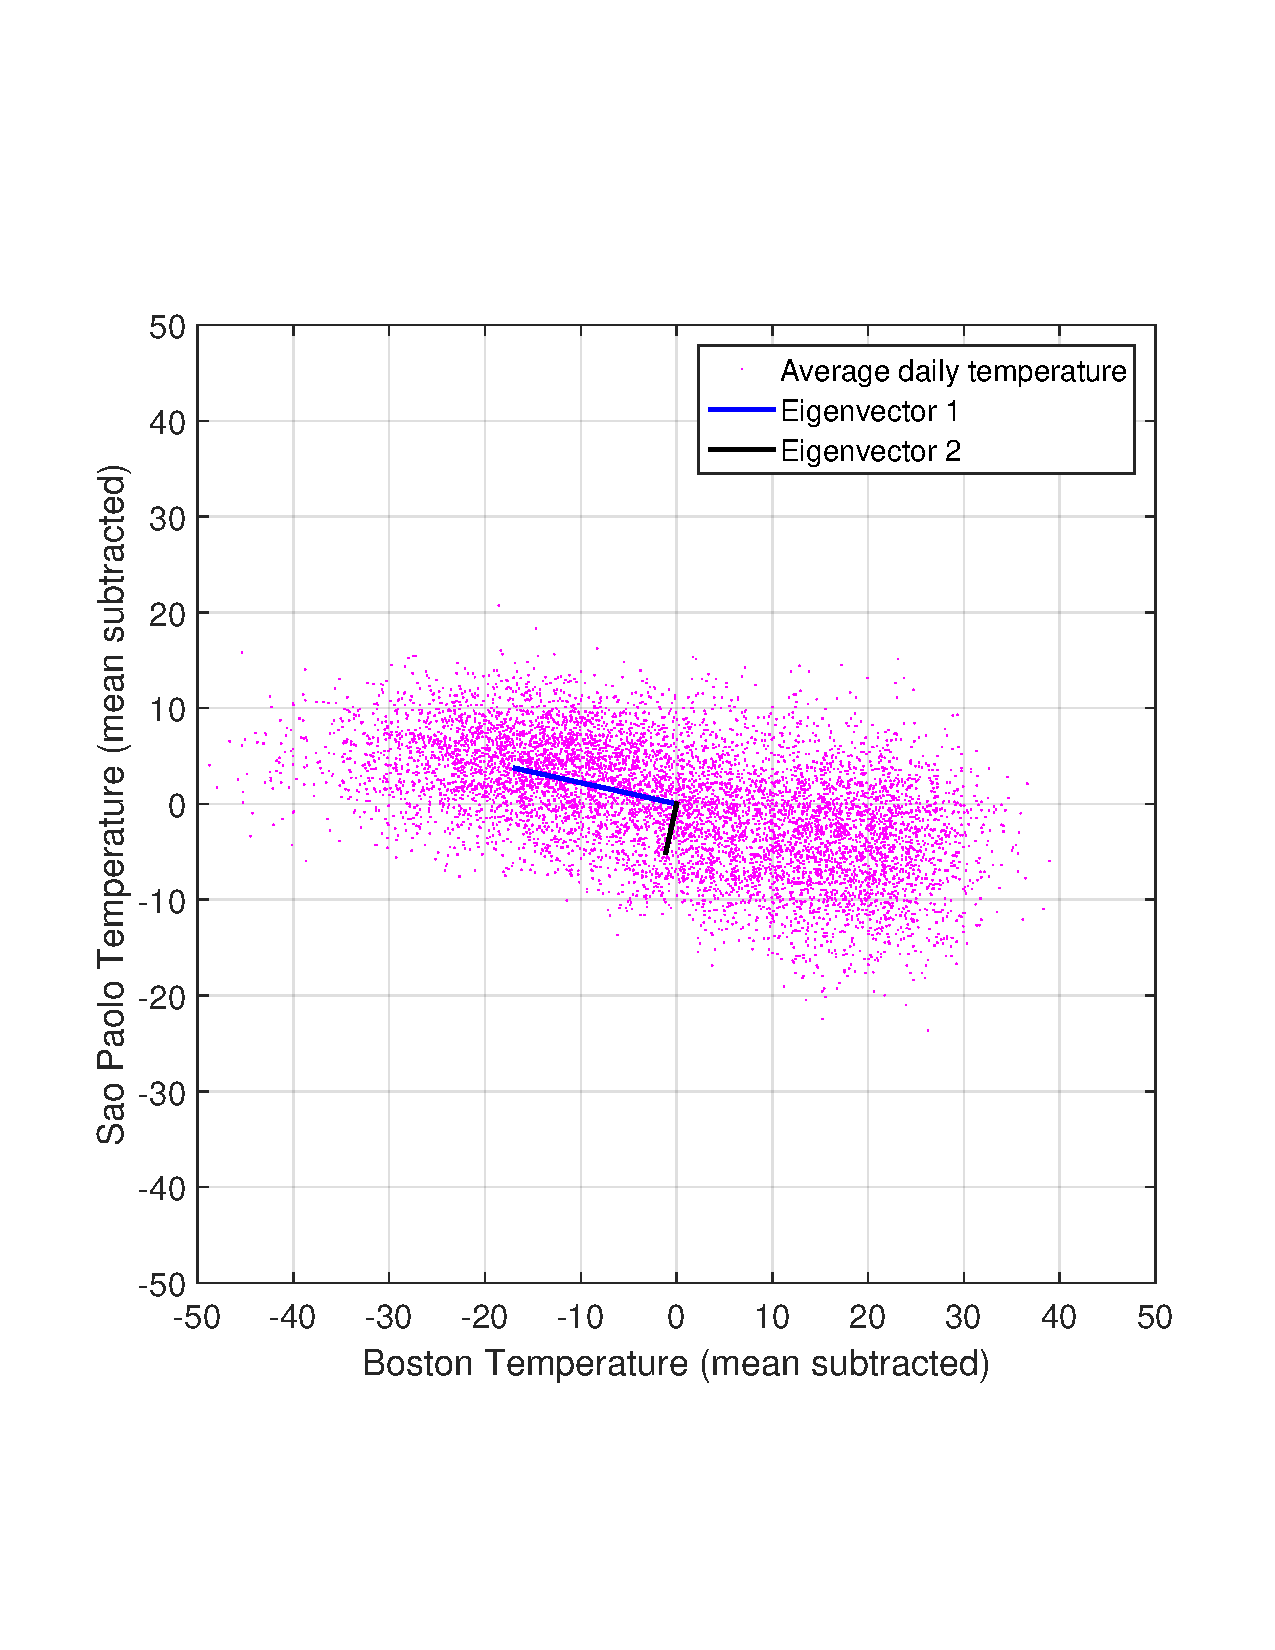
\includegraphics[width=0.45\textwidth]{FacesNight5/figs/BostonSaoPaoloCentered.pdf}
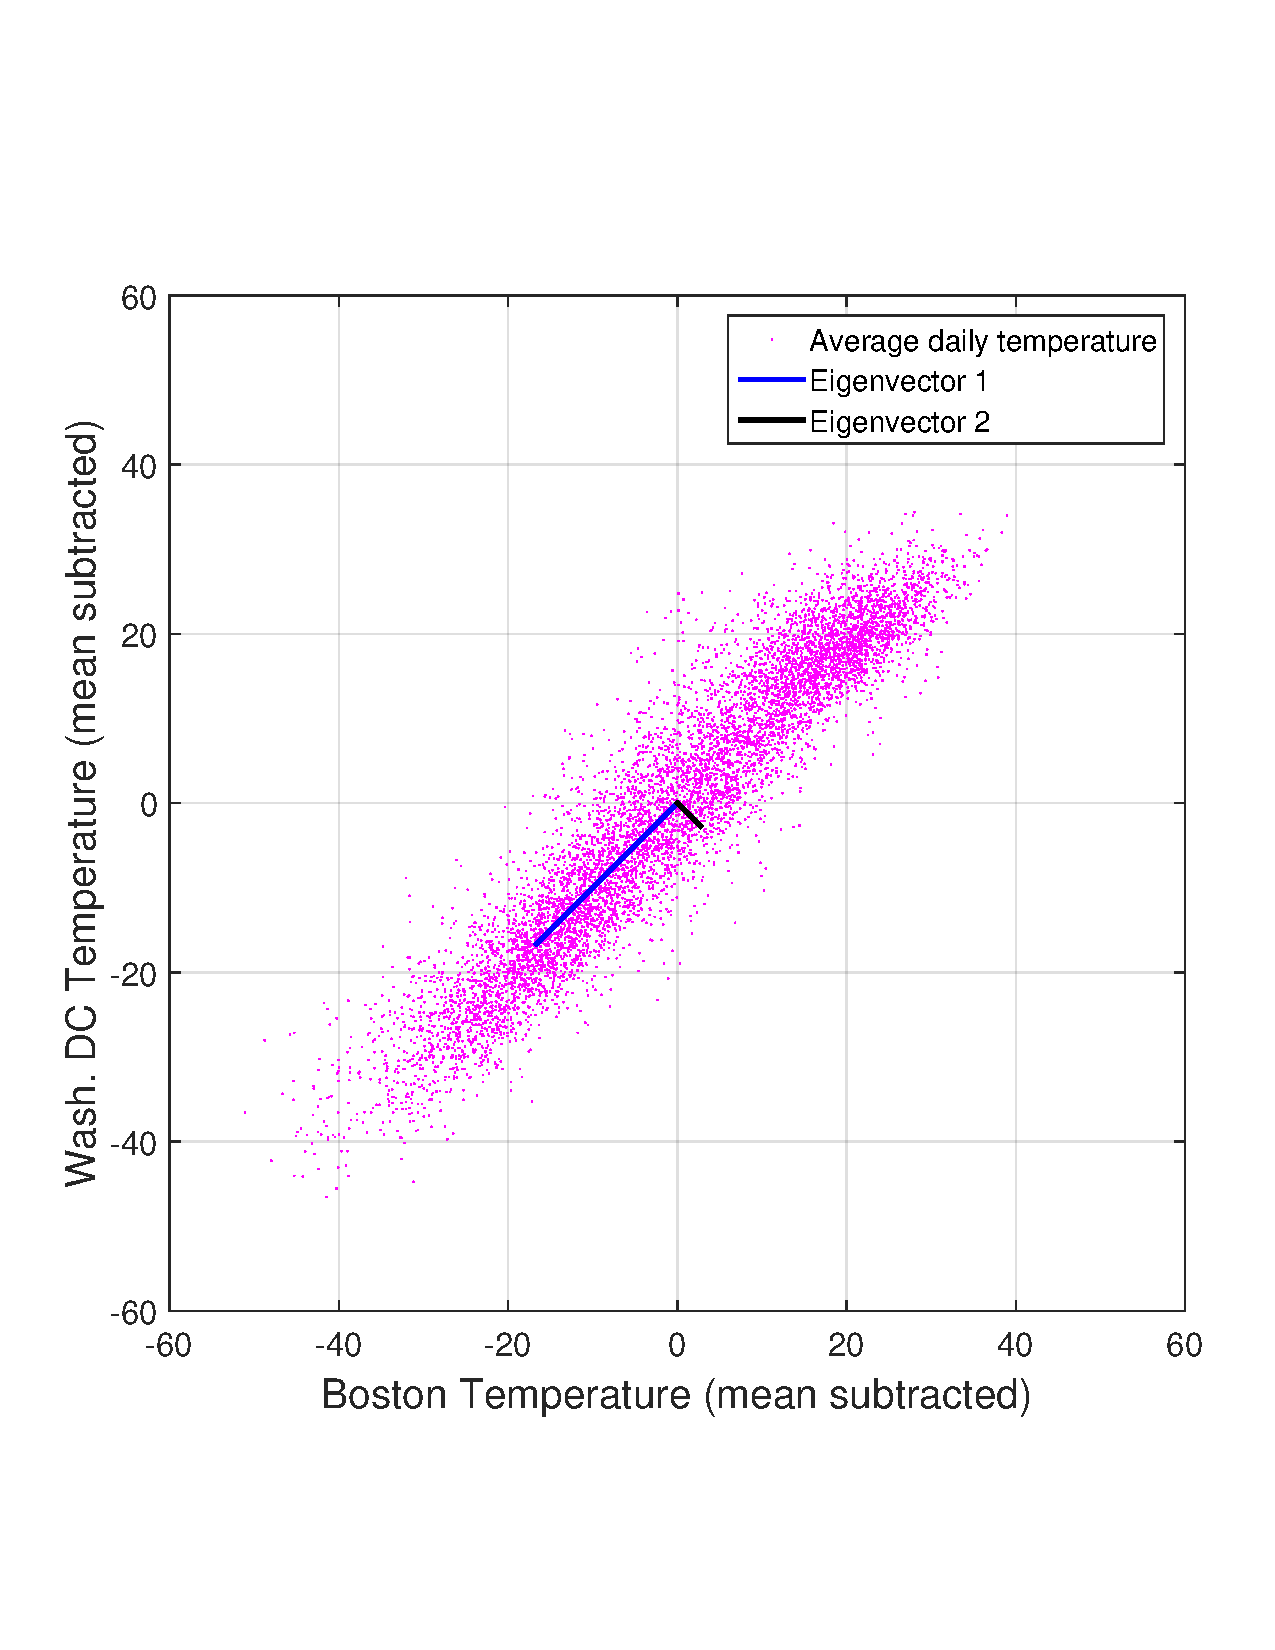
\includegraphics[width=0.45\textwidth]{FacesNight5/figs/BostonWashingtonCentered.pdf}
\captionof{figure}{Centered average daily temperatures of Boston vs Sao Paolo (left) and Boston vs Washington DC, with the eigenvectors of the covariance matrix. }
\label{figBostonWashington}
\end{center}

From visually inspecting these figures we saw that eigenvector 1, which corresponded to the larger of the two eigenvalues, seemed to be pointing in the direction where the data exhibited the most variability (i.e., the data was most spread out along this direction).  You also looked at this for a 3D dataset consisting of the temperatures from Boston, Sao Paolo, and Washington DC.

\begin{center}
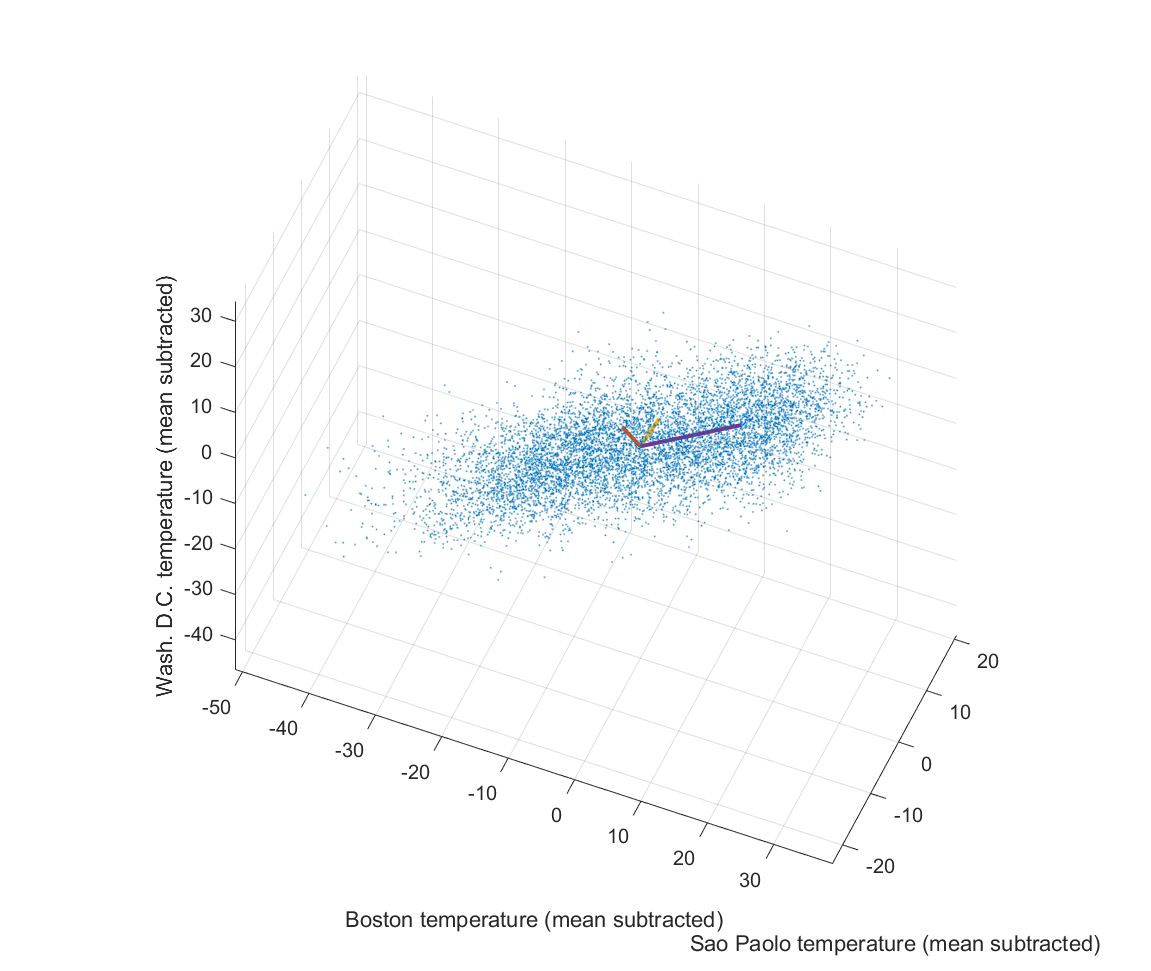
\includegraphics[width=0.45\textwidth]{FacesNight6/figs/tempplot.png}
\captionof{figure}{Temperatures and eigenvectors for Boston, Sao Paolo, and Washington DC}
\label{temps}
\end{center}

In this 3D dataset, we see the same phenomenon: that the principal eigenvector points along the direction of maximum variation in the data.  It turns out that this phenomenon will hold no matter the dimensionality of the data (it works for 4D datasets, 10D datasets, and even datasets with 1,000s of dimensions)!  This fact provides the basis for the principal components algorithm.  In PCA, instead of working with the data in its original form, we express it in a basis given by eigenvectors of the covariance matrix that have the largest eigenvalues. We can understand the properties of using this basis through two key properties.

\begin{itemize}
\item \emph{Property 1}: the principal eigenvectors of the covariance matrix will maximize the variance of the data when the data is projected onto these vectors (we can think of vectors that capture large variation in the data as representing important properties of the data).
\item \emph{Property 2}: the principal eigenvectors of the covariance matrix will allow us, in a particular sense, to optimally compress our data.  That is, we will be able to recover the original data with the highest possible accuracy from the projections of the data onto the principal eigenvectors.
\end{itemize}

The power of PCA lies in its ability to achieve both of the properties described above simultaneously.  For this reason, the principal components of a dataset will act as keys to unlocking the secrets lurking in the data!  \textbf{Today we will be exploring property 1, and in the night assignment you will also be exploring property 2}.

\subsection{The Principal Eigenvector as the Direction of Maximum Variance}

The graphs of the daily temperature data show, graphically, that the principal eigenvector of the covariance matrix corresponds to the direction of maximum variation in the data.  In this section we'll be formalizing this result.  We've decided to structure this part of the day assignment as an extended exercise where you will be working through the proof of this fact step-by-step.  While there are many ways to do this proof, we'll be walking you through one way that will connect well with the ideas we've been exploring in the last week or so of the course.  We recommend that you do a part of the proof, check it against the solutions and then move onto the next piece.

Before getting started, let's look at some material from night 6 that shows that the covariance matrix can be computed using matrix multiplication.

\begin{quote}
Suppose that  we have two different data variables $x$ and $y$ (e.g. corresponding to temperatures in Boston and Sao Paolo), with $x_i$ and $y_i$ being different values in the data set we can define a a matrix $\mathbf{A}$ as follows:

\begin{align}
\mathbf{A} = \frac{1}{\sqrt{N-1}} \begin{pmatrix}
    {x_1-\mu_x} & {y_1-\mu_y}\\
   {x_2-\mu_x} &  {y_2-\mu_y}\\
    {x_3-\mu_x} & {y_3-\mu_y}\\
    \vdots & \vdots \\
    x_N - \mu_x & y_N - \mu_y
  \end{pmatrix} \label{eq:covar}
\end{align}
where $\mu_x$ is the mean  of the first column, and $N$ is the number of samples (rows).  The covariance matrix of $x$ and $y$ is $\mathbf{R} = \mathbf{A}^T \mathbf{A}$. You can think of the entries of this matrix as storing the un-normalized correlations between the temperatures. Because $\mathbf{R}^T = \mathbf{R}$, this matrix is symmetric, and hence has orthogonal eigenvectors.
\end{quote}

Let's assume that we are given a dataset with $n$ samples and $d$ dimensions (instead of just 2 dimensions as shown above).  We can transform it into the form given in Equation~\ref{eq:covar} by subtracting the mean from each column and dividing the entire matrix by $\sqrt{N-1}$.  We now have a mean-centered data matrix $\A$ with $n$ rows and $d$ columns and the covariance matrix of our data is given by $\A^\top \A$.


\begin{prob}
Our overall goal is to show that if we take a unit vector $\u$, project our mean-centered data onto it (as $\A \u$), and examine the variance of the projected data, that this variance is largest when $\u$ is the principal eigenvector of the covariance matrix $\A^\top \A$.

\begin{enumerate}
\item First we'll write down an expression for the variance of $\A \u$ (we'll write this as $Var[ \A \u]$) as a matrix multiplication.  We'll do this step together (i.e., we'll show you how to do it).  For this part of the exercise you should make sure you understand the steps we performed.

If $\A$ is in the form given in Equation~\ref{eq:covar}, then $\A \u$ will have 0 mean (since $\A \u$ is a linear combination of columns with 0 mean).  Using the same logic that led us to conclude that $\A^\top \A$ is the covariance matrix of the data, $(\A \u)^\top (\A \u)$ will give us the variance of the data projected onto $\u$ (remember that variance is just a special case of covariance where we are comparing a quantity to itself).  It's worth noting that since $\A \u$ is a vector, the expression $(\A \u)^\top (\A \u)$ is known as the inner product, which is really the same as the dot product (that is, $(\A \u)^\top (\A \u) = \A \u \cdot \A \u$).  Thus, the variance is given by the following equation.

\begin{align*}
Var[\A \u] &= (\A \u)^\top (\A \u) \\
&= \u^\top \A^\top \A \u ~~~~~\mbox{note: we are applying the rule that } (\A\B)^\top = \B^\top \A^\top
\end{align*}

\item Substitute  the eigenvalue decomposition,  $\mathbf{V} \mathbf{D} \mathbf{V}^\top$,  for the covariance matrix $\A^\top \A$ (since $\A^\top \A$ is symmetric and real, we can substitute $\mathbf{V}^\top$ for the inverse of $\mathbf{V}$ in the eigenvalue decomposition).

\item Define the vector $\y = \mathbf{V}^\top \u$ and substitute it into the expression from part 2.

\item Expand out the expression in part 3 so that it is in terms of the squares of the elements of $\y$ and the diagonal entries of $\mathbf{D}$ in order of largest to smallest.

\item Show that $\y$ is a unit vector by taking the inner product with itself and showing that it is equal to 1 (recall that the inner product is the same as the dot product).  \emph{Hint: $\mathbf{V} \mathbf{V}^\top = \mathbf{I}$ since $\mathbf{V}$ is orthonormal and has $d$ linearly independent columns.}

\item Argue that since $\y$ is a unit vector (which implies $\sum_{i=1}^d y_i^2 = 1$), that the expression in part 4 is maximized when $y_i = 1$ when $i$ is the index of the principal eigenvector and $y_i = 0$ when $i$ is any other index.  To get a feel for why this is true, try writing out a specific case where, perhaps, $\y$ has two or three dimensions.

\item Show that we achieve the value of $\y$ in part 5 (that is where $y_i = 1$ when $i$ is the index of the principal eigenvector and $y_i = 0$ when $i$ is any other index) when $\u$ is the principal eigenvector of $\A^\top \A$.

\item What have you just shown?!?  Make sure you have a sense of what you just did (don't get lost in the mathematical symbols).

\end{enumerate}

\end{prob}
\begin{sol}
\be
\item Solution is already given in the problem
\item 
\begin{align*}
Var[\A \u] &=\u^\top \mathbf{V} \mathbf{D} \mathbf{V}^\top \u
\end{align*}

\item 
\begin{align*}
Var[\A \u] &= (\mathbf{V}^\top \u)^\top \mathbf{D} (\mathbf{V}^\top \u) \\
&= \y^\top \mathbf{D} \y
\end{align*}

\item
\begin{align*}
Var[\A \u] &= \y^\top \mathbf{D} \y \\
&= \y^\top \begin{bmatrix} y_1 D_{1,1} \\  y_2 D_{2,2} \\ \vdots \\ y_d D_{d,d} \end{bmatrix} \\
&= \sum_{i=1}^d y_i^2 D_{i,i}
\end{align*}


\item
\begin{align*}
\y^\top \y &= (\mathbf{V}^\top \u)^\top (\mathbf{V}^\top \u) \\
&= \u^\top \mathbf{V} \mathbf{V}^\top \mathbf{u} \\
&= \u^\top  \mathbf{u} \\
&= 1
\end{align*}


\item If we choose $y_i = 1$ where $i$ is the index of the principal eigenvector, then the expression in part 4 will give us $D_{i,i}$.  Any other choice of $\y$ will result in some weighted combination of the eigenvalues (the diagonal elements of $\mathbf{D}$) where the weights are all positive and add up to 1.  It is easy to see that putting any weight on a non-maximal eigenvalue will result in a lower variance as computed by the expression in part 4.


\item Since $\y = \mathbf{V}^\top \u$, $y_i$ is the dot product of $\u$ and the $i$th eigenvector, $\mathbf{v_i}$, with $\u$.  Since we assume all of the eigenvectors are unit vectors and mutually orthogonal, if we set $\u$ to be the principal eigenvector of $\A^\top \A$, then the dot product of $\u$ and $\mathbf{v_i}$ will be 1 for $i$ corresponding to the principal eigenvector and 0 for all other indices.

\item You just showed that the direction along the principal eigenvector of the covariance matrix maximizes the variance of the projected data.  That's pretty cool!

\ee
\end{sol}

\subsection{Beyond the first principal component}

We've now gone into depth in understanding the first principal component and its amazing property of maximizing variance.  The second principal component is simply going to be the direction that maximizes variance subject to the requirement that it is orthogonal to the first principal component.  With a slight modification to your proof you can show that the second principal component will be in the direction of the eigenvector with the second largest eigenvalue.  The trend continues for other principal components (i.e., the $i$th principal component is the eigenvector with the $i$th largest eigenvalue).

\subsection{Applications of PCA (thinking it through conceptually)}

In this section you're going to be thinking about what the PCA algorithm might do when applied in different domains.  The focus of this section will be on trying to understand at a conceptual level what might happen when we apply PCA.  In the next section, you'll be reading through an example of applying PCA to some actual data.

\begin{prob}
For each application, hypothesize what the first principal component might be.  That is, for each particular scenario what would the direction be that maximizes the variance of the data projected onto that direction?  What might the second principal component be (that is a vector orthogonal to the first that maximizes the variance of the data)?

\begin{enumerate}
\item Consider a dataset consisting of ratings from $n$ users of $m$ movies.  Let's assume that the ratings are numerical and are on a scale of 1 to 5 (5 being the best).  Consider some collection of movies (they could be some specific movies or you could just think of movie genres) and a particular population of users (could be college students, QEA professors, or just the general population).  Draw the data matrix $\A$ and label the rows and columns (e.g., with movies or users).  In a qualitative sense, make a prediction as to what the first principal component would look like for this dataset.  What might the second principal component look like?  No numbers... just guess at which dimensions would be positive, negative, or close to 0 for your principal components.

\item Consider a dataset consisting of the prevalence of the flu in various parts of the US.  The CDC maintains an animated map of the flu activity over time, which you can (and should) access at \url{https://www.cdc.gov/flu/weekly/usmap.htm}.  To simplify this data, let's think about the number of flu cases in each of the six major major geographical regions of the US.

\begin{center}
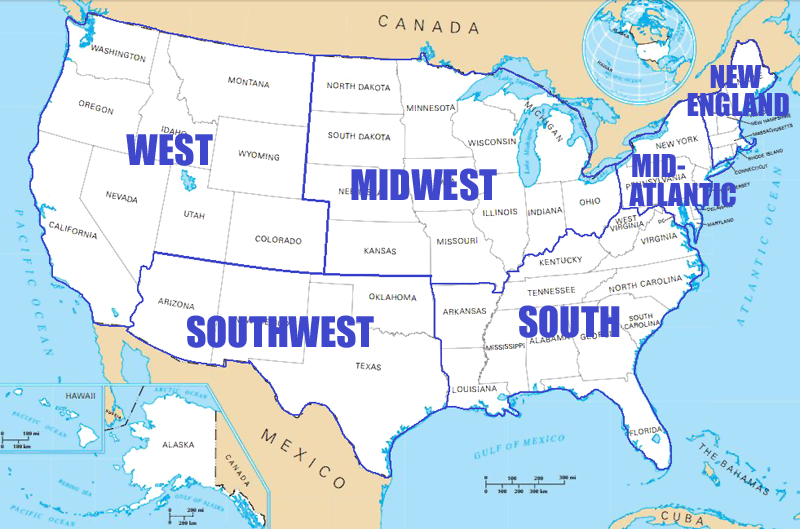
\includegraphics[width=0.6\linewidth]{FacesDay7/figs/USRegionMap.png}
\end{center}

If we think about our data matrix as consisting of a row for each week of measured flu activity and each column as a region of the US, in a qualitative sense, make a prediction as to what the first principal component would look like for this dataset.  What might the second principal component look like?  No numbers... just guess at which dimensions would be positive, negative, or close to 0 for your principal components.

\end{enumerate}
\end{prob}

\begin{prob}
With your table-mates, read through this post that shows \href{https://nycdatascience.com/blog/student-works/figuring-out-american-politics-so-easy-a-computer-can-do-it/}{the application of PCA to understanding the US political leanings} (if you are viewing this in DropBox preview and can't click the link, go to \url{http://bit.ly/37n9qwe}).  Before, starting here are some process suggestions.

\bi
\item Checkin with folks at your table as to how they'd like to go through this document (e.g., read the entire thing individually and come together and ask questions, read it individually but stop after each major section to ask questions, read it aloud as a table).
\item If you don't understand something, you can either call over an instructor or note your confusion on the whiteboard and keep going (e.g., if its something that doesn't impede your understanding of the main points in the article).
\ei

\end{prob}

\pagebreak
\shipoutAnswer

